\section{Visualise attention mechanism}

An important part of analysing the data is the attention mechanism, which allows the model to focus on different parts of the input data. Being able to visualise this mechanism is a key aspect of understanding how the network behaves. In this notebook I will

\begin{itemize}
\item Load preselected data
\item Run the model on the preselected data
\item Visualise the attention map on the input data
\end{itemize}

Due to the size of the network, this image has been saved. Uncomment the code to reproduce.

\begin{verbatim}
from libs.network.network import AttU_Net
import pickle
import os
import torch
import matplotlib.pyplot as plt
import torch.nn.functional as F

# uncomment when running the model independently

# # Define paths
# network_path = "data/network_att_map.pth"
# data_path = "data/data_att_map.pkl"

# # load torch input tensor
# with open(data_path, "rb") as f:
#     input_tensor = pickle.load(f)


# load saved data
with open("data/attention_overlay.pkl", "rb") as f:
    data = pickle.load(f)
    input_tensor = data["input_tensor"]
    attention = data["attention"]
\end{verbatim}

\subsubsection{Load network and run output}

\begin{verbatim}
# network = AttU_Net()
# network.load_state_dict(torch.load(network_path, map_location=torch.device('cpu')))  # Load the trained network weights
# network.eval()

# output, attention_maps = network.getAttenuationMap(input_tensor)
\end{verbatim}

\subsection{Visualise attention mechanism}

Define function show\_attention\_overlay which as an argument takes the input data, the attention weights, the slice axis and the slice index.
For this example I have chosen to slice along the y-direction to properly visualise the sinogram.

\begin{verbatim}
def show_attention_overlay(input_tensor, attention, slice_axis=2, slice_idx=0, title="Attention Overlay"):
    """
    Visualize attention over an input slice.

    Args:
        input_tensor: torch.Tensor [1, C, D, H, W]
        attention:    torch.Tensor [1, 1, D', H', W']
        slice_axis:   0=D, 1=H, 2=W (which axis to slice through)
        slice_idx:    index along that axis
    """
    assert input_tensor.ndim == 5 and attention.ndim == 5

    # Resize attention to match input spatial dims
    attn_resized = F.interpolate(attention, size=input_tensor.shape[2:], mode='trilinear', align_corners=False)

    # Select first input channel and remove batch dim
    input_tensor = input_tensor[6, 0].detach().cpu()
    attn_tensor = attn_resized[6, 0].detach().cpu()
    
    # Normalize attention
    attn_tensor = (attn_tensor - attn_tensor.min()) / (attn_tensor.max() - attn_tensor.min() + 1e -8)

    # Choose slice
    if slice_axis == 0:  # Depth
        input_slice = input_tensor[slice_idx, :, :].numpy()
        attn_slice  = attn_tensor[slice_idx, :, :].numpy()
    elif slice_axis == 1:  # Height
        input_slice = input_tensor[:, slice_idx, :].numpy()
        attn_slice  = attn_tensor[:, slice_idx, :].numpy()
    elif slice_axis == 2:  # Width
        input_slice = input_tensor[:, :, slice_idx].numpy()
        attn_slice  = attn_tensor[:, :, slice_idx].numpy()
    else:
        raise ValueError("slice_axis must be 0 (D), 1 (H), or 2 (W)")

    plt.figure(figsize=(10, 4))
    plt.rcParams['axes.labelsize'] = 14

    # Plot overlay
    plt.imshow(input_slice, cmap='gray')
    plt.imshow(attn_slice, cmap='jet', alpha=0.3)
    # make colourbar same height as image
    plt.xlabel('Z')
    plt.ylabel('X')
    plt.colorbar(label=r'$\alpha$', fraction=0.046, pad=0.04)
    plt.show()
\end{verbatim}

\subsubsection{Plot attention map}

\begin{verbatim}
# attention = attention_maps['att2']
show_attention_overlay(input_tensor, attention, slice_axis=1, slice_idx=41, title="Attention from att4")
\end{verbatim}

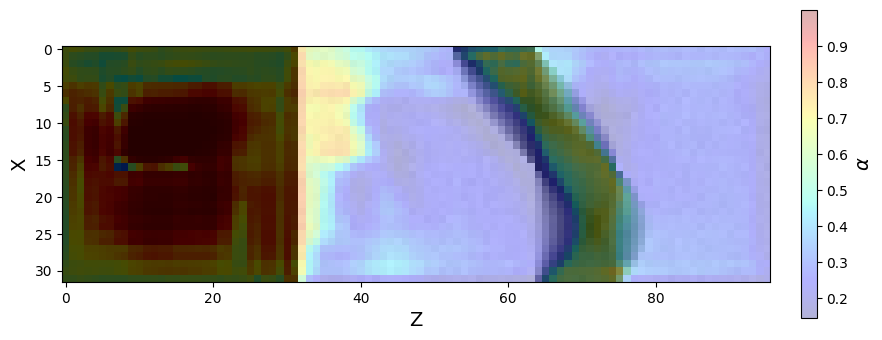
\includegraphics[width=0.7\linewidth]{files/a3bbbb4f0e549cbc4292afd07287ad34.png}

\begin{verbatim}

\end{verbatim}